\documentclass[a4paper]{article}
\usepackage[utf8]{inputenc}
\usepackage{todonotes}
\usepackage[russian]{babel}
\usepackage{graphicx}
\usepackage{float}
\usepackage{wrapfig}
\usepackage{tikz}
\usepackage{amsmath, amssymb}
\usepackage{hyperref}
\usepackage{listings}
\usepackage{caption}
\usepackage{geometry}
\usepackage{fancyhdr}
\usepackage{nicefrac}
\usepackage{xcolor}
\geometry{left=2cm,right=2cm,top=2cm,bottom=2cm}
\definecolor{urlcolor}{rgb}{0,0,1}
\definecolor{linkcolor}{rgb}{0,0,0.8}
\hypersetup{pdfborder=0 0 0}
\hypersetup{pdfstartview=FitH, linkcolor=linkcolor, urlcolor=urlcolor, colorlinks=true}

\definecolor{strings}{rgb}{0,0.6,0}
\definecolor{comments}{rgb}{0,0.3,0}
\definecolor{numbers}{rgb}{0.5,0.5,0.5}
\definecolor{keywords}{rgb}{0.09,0.61,0.95}
\definecolor{background}{rgb}{0.97,0.97,0.97}

\lstdefinestyle{codestyle}{
    backgroundcolor=\color{background},
    commentstyle=\color{comments},
    keywordstyle=\color{keywords},
    stringstyle=\color{strings},
    numberstyle=\tiny\color{numbers},
    basicstyle=\ttfamily\footnotesize,
    breakatwhitespace=false,
    breaklines=true,
    captionpos=b,
    inputencoding=utf8,
    keepspaces=true,
    numbers=left,
    numbersep=5pt,
    showspaces=false,
    showstringspaces=false,
    showtabs=false,
    tabsize=2,
    extendedchars=true
}

\lstset{style=codestyle}

\newcommand{\addsection}[1]{
    \phantomsection
    \addcontentsline{toc}{section}{#1}
    \section*{#1}
}
\newcommand{\addsubsection}[1]{
    \phantomsection
    \addcontentsline{toc}{subsection}{#1}
    \subsection*{#1}
}
\newcommand{\addsubsubsection}[1]{
    \phantomsection
    \addcontentsline{toc}{subsubsection}{#1}
    \subsubsection*{#1}
}

\begin{document}

% Титульный лист
\begin{titlepage}
    \centering
    {\large Федеральное государственное автономное образовательное учреждение\par}
    {\large высшего образования\par}
    {\bfseries САНКТ-ПЕТЕРБУРГСКИЙ НАЦИОНАЛЬНЫЙ ИССЛЕДОВАТЕЛЬСКИЙ УНИВЕРСИТЕТ ИТМО\par}
    {\bfseries Факультет систем управления и робототехники\par}
    \vfill
    {\Large \bfseries Лабораторная работа №4\par}
    {\Large \bfseries Линейная фильтрация\par}
    \vfill
    
    \begin{flushright}
        Студент: Сайфуллин Д.Р. \\
        Поток: ЧАСТ.МЕТ. R23 1.5 \\ 
        Преподаватели: Перегудин А.А.\\
        Догадин  Е.В.
    \end{flushright}
    \vfill
    Санкт-Петербург \\
    2025 г.
\end{titlepage}

% Оглавление
\tableofcontents
\newpage

\addsection{Задание 1. Линейные фильтры}
\addsubsection{Фильтр первого порядка}
Для выполнения задания, как и в прошлой лабораторной работе, необходимо задать параметры \(a, t_1, t_2\) и рассмотреть предложенную функцию. Пусть параметры \(a = 2, t_1 = 2, t_2 = 6\), функция нашего сигнала будет:
\[g(t)=
\begin{cases}
    2, & t \in [2, 6],\\[1ex]
    0, & \text{иначе}.
\end{cases}\]
\noindent
Также нужно задать зашумлённую версию нашего сигнала, которая имеет вид:
\[
u(t)=g(t)+b\,\xi(t)+c\sin{dt},
\]
где \(\xi(t)\) – белый шум (равномерно распределённый на \([-1,1]\)), а \(b, c, d\) --- параметры возмущения.

При выполнении этого пункта гармоническая составляющая отсутствует (\(c=0\)). Таким образом к исходному сигналу добавляется только белый шум с коэффициентом $b$. Сигнал принимает вид:
\[u(t) = g(t) + b \cdot \xi(t),\]
где $\xi(t)$ --- белый шум, равномерно распределённый на интервале $[-1,1]$. Параметр $b$ зададим как $b = 0.5$. Для исследования влияния параметра постоянной времени \(T\) проводились эксперименты при различных значениях \(T\): 0.1, 0.5, 1.0 и 2.0. Для каждого эксперимента были построены следующие графики:
\begin{enumerate}
    \item Временные сигналы: исходный \(g(t)\), зашумлённый \(u(t)\) и фильтрованный \(y(t)\).
    \item Фурье-образы сигналов.
    \item Амплитудно-частотная характеристика (АЧХ) фильтра.
    \item Сравнение временных сигналов, полученных методом \texttt{lsim} и через обратное Фурье-преобразование.
    \item Сравнение Фурье-образов фильтрованного сигнала и произведения передаточной функции на спектр зашумлённого сигнала.
\end{enumerate}

Перйдем к анализу и сравнению полученных результатов.
\begin{figure}[H]
    \centering
    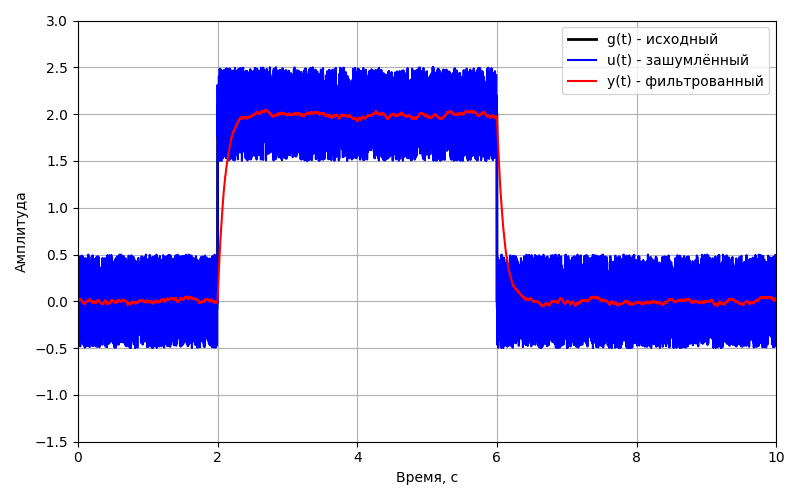
\includegraphics[width=0.8\textwidth]{src/task_1_1/time_2.0_0.1.png}
    \caption{Временные сигналы при \(T=0.1\).}
    \label{fig:time_0.1}
  \end{figure}
\noindent На рисунке~\ref{fig:time_0.1} представлены временные сигналы для \(T=0.1\). Фильтрованный сигнал (красная линия) демонстрирует небольшой эффект сглаживания, однако шумовые компоненты остаются достаточно выраженными. Это свидетельствует о том, что при малом значении \(T\) фильтр имеет быстрый отклик, но недостаточно эффективно подавляет высокочастотные колебания.

\begin{figure}[H]
  \centering
  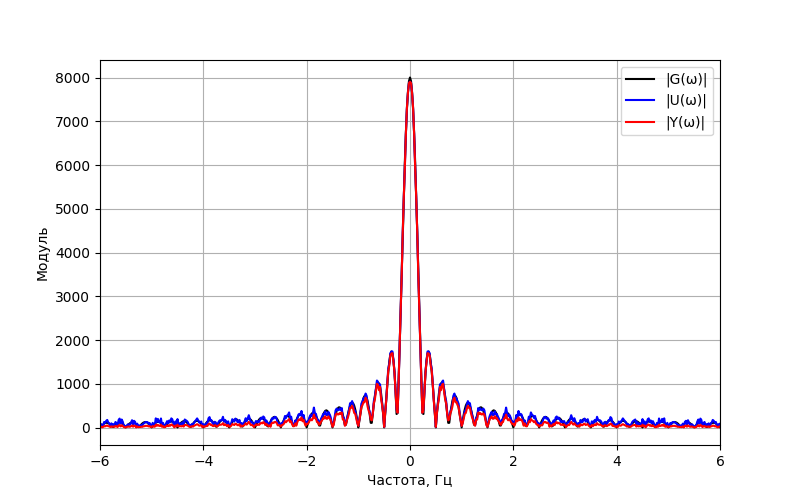
\includegraphics[width=0.8\textwidth]{src/task_1_1/spec_2.0_0.1.png}
  \caption{Спектральные образы сигналов при \(T=0.1\).}
  \label{fig:spec_0.1}
\end{figure}
\noindent Рисунок~\ref{fig:spec_0.1} демонстрирует спектральные образы сигналов для \(T=0.1\). Исходный сигнал имеет спектр, характерный для прямоугольного импульса, а добавление шума приводит к появлению дополнительных высокочастотных компонентов. Фильтрованный сигнал сохраняет низкочастотную составляющую, а высокочастотные компоненты остаются слабо подавленными.

\begin{figure}[H]
    \centering
    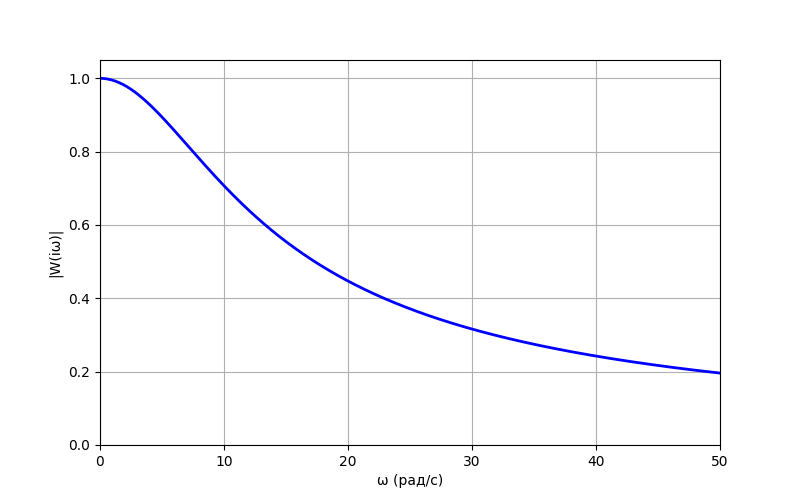
\includegraphics[width=0.8\textwidth]{src/task_1_1/ach_2.0_0.1.png}
    \caption{АЧХ фильтра при \(T=0.1\).}
    \label{fig:ach_0.1}
\end{figure}
\noindent Рисунок~\ref{fig:ach_0.1} иллюстрирует амплитудно-частотную характеристику (АЧХ) фильтра для \(T=0.1\). При \(\omega=0\) модуль передаточной функции равен 1, а с ростом \(\omega\) значение \(|W(i\omega)|\) стремительно убывает. При малом \(T\) спад происходит на относительно высоких частотах, что объясняет недостаточное подавление высокочастотного шума, наблюдаемое на спектральных графиках.

\begin{figure}[H]
    \centering
    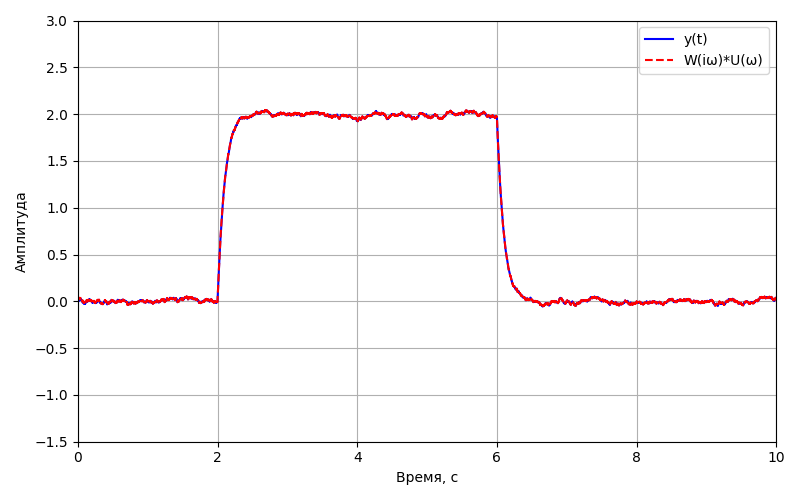
\includegraphics[width=0.8\textwidth]{src/task_1_1/time_comp_2.0_0.1.png}
    \caption{Сравнение временных сигналов для \(T=0.1\).}
    \label{fig:timecomp_0.1}
\end{figure}
\noindent Рисунок~\ref{fig:timecomp_0.1} демонстрирует сравнение временных сигналов, полученных методом \texttt{lsim} и посредством обратного Фурье-преобразования умноженного спектра. Для \(T=0.1\) наблюдается хорошее совпадение обеих кривых, что подтверждает корректность реализации фильтрации как в временной, так и в частотной областях.

\begin{figure}[H]
    \centering
    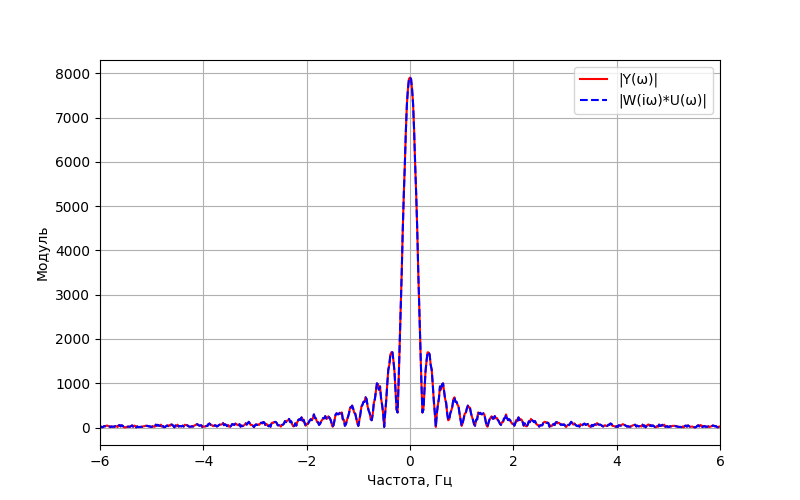
\includegraphics[width=0.8\textwidth]{src/task_1_1/spec_comp_2.0_0.1.png}
    \caption{Сравнение спектральных образов для \(T=0.1\).}
    \label{fig:speccomp_0.1}
\end{figure}
\noindent На рисунке~\ref{fig:speccomp_0.1} представлено сравнение Фурье-образов фильтрованного сигнала и произведения спектра зашумлённого сигнала на передаточную функцию \(W(i\omega)\) для \(T=0.1\). Графики совпадают, что дополнительно подтверждает правильность выбранного метода фильтрации.

\begin{figure}[H]
    \centering
    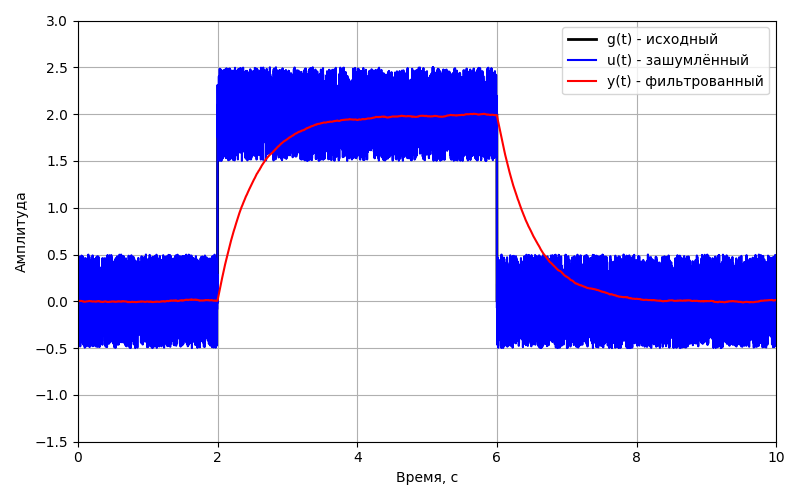
\includegraphics[width=0.8\textwidth]{src/task_1_1/time_2.0_0.5.png}
    \caption{Временные сигналы при \(T=0.5\).}
    \label{fig:time_0.5}
\end{figure}
\noindent При увеличении значения \(T\) до 0.5 и 1.0 наблюдаются существенные изменения. Рисунки для \(T=0.5\) (см. рисунки \ref{fig:time_0.5}--\ref{fig:speccomp_0.5}) показывают, что фильтр начинает более эффективно сглаживать сигнал. Временные графики демонстрируют уменьшение амплитуд шума, а спектральный анализ свидетельствует о более заметном ослаблении высокочастотных компонент. Однако наблюдается небольшая задержка пика, что является следствием увеличения времени реакции фильтра.

\begin{figure}[H]
  \centering
  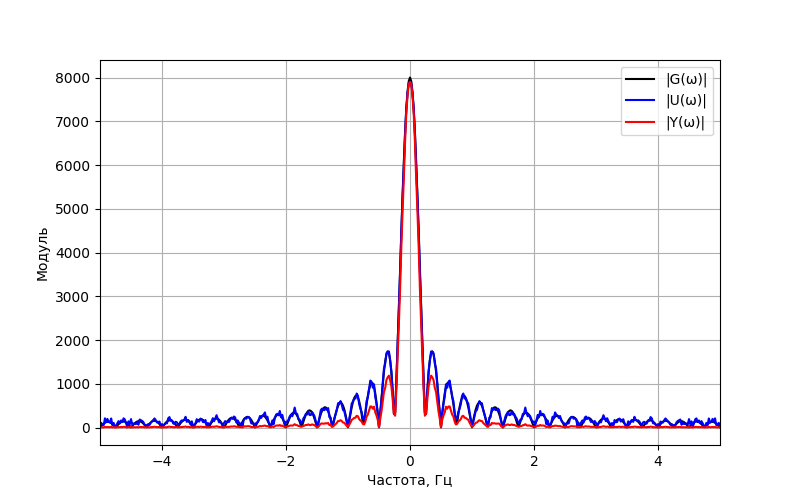
\includegraphics[width=0.8\textwidth]{src/task_1_1/spec_2.0_0.5.png}
  \caption{Спектральные образы сигналов при \(T=0.5\).}
  \label{fig:spec_0.5}
\end{figure}

\begin{figure}[H]
  \centering
  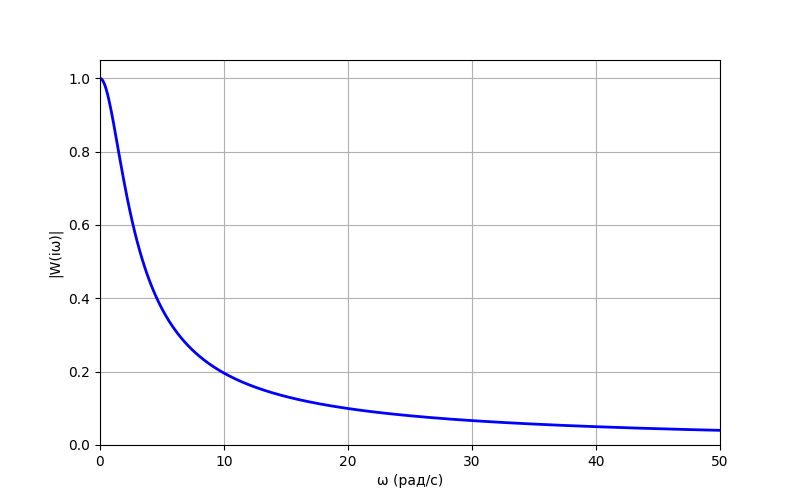
\includegraphics[width=0.8\textwidth]{src/task_1_1/ach_2.0_0.5.png}
  \caption{АЧХ фильтра при \(T=0.5\).}
  \label{fig:ach_0.5}
\end{figure}

\begin{figure}[H]
  \centering
  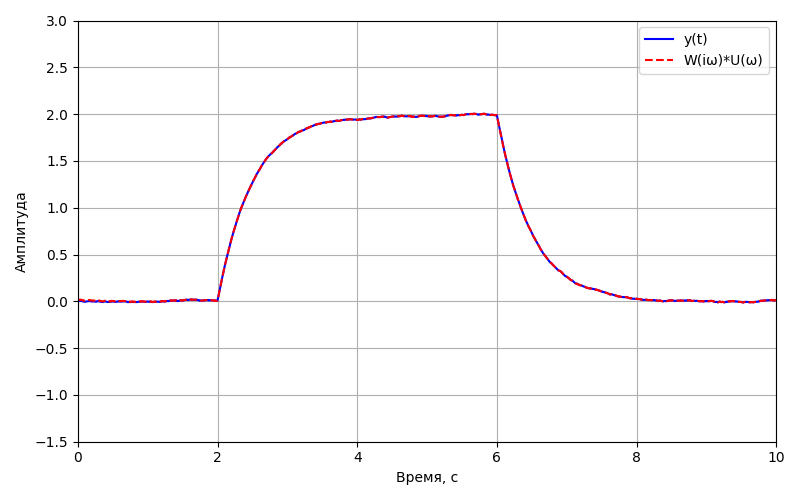
\includegraphics[width=0.8\textwidth]{src/task_1_1/time_comp_2.0_0.5.png}
  \caption{Сравнение временных сигналов для \(T=0.5\).}
  \label{fig:timecomp_0.5}
\end{figure}

\begin{figure}[H]
  \centering
  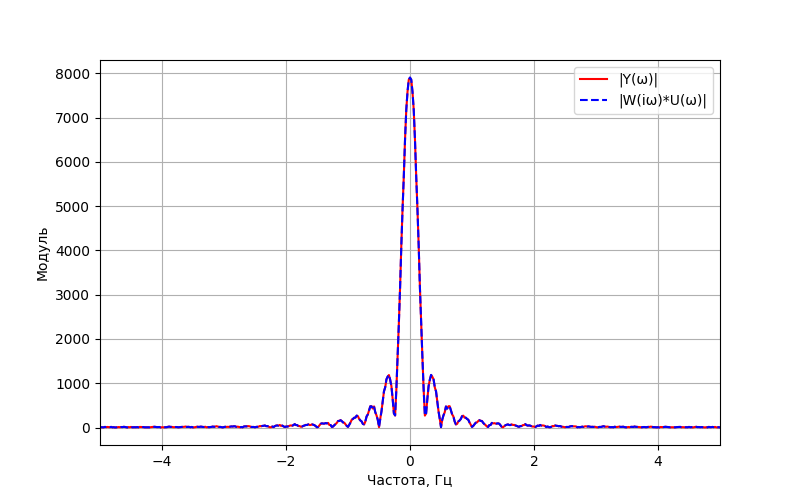
\includegraphics[width=0.8\textwidth]{src/task_1_1/spec_comp_2.0_0.5.png}
  \caption{Сравнение спектральных образов для \(T=0.5\).}
  \label{fig:speccomp_0.5}
\end{figure}

При \(T=1.0\) наблюдается ещё более выраженное сглаживание сигнала. Временные графики (см. рисунок~\ref{fig:time_1.0}) показывают, что пиковая область сигнала становится более вытянутой, что свидетельствует о задержке отклика фильтра. Спектральные графики демонстрируют, что высокочастотные компоненты практически исчезают, а АЧХ фильтра (рисунок~\ref{fig:ach_1.0}) убывает более плавно с уменьшением частотного диапазона пропускания.

\begin{figure}[H]
  \centering
  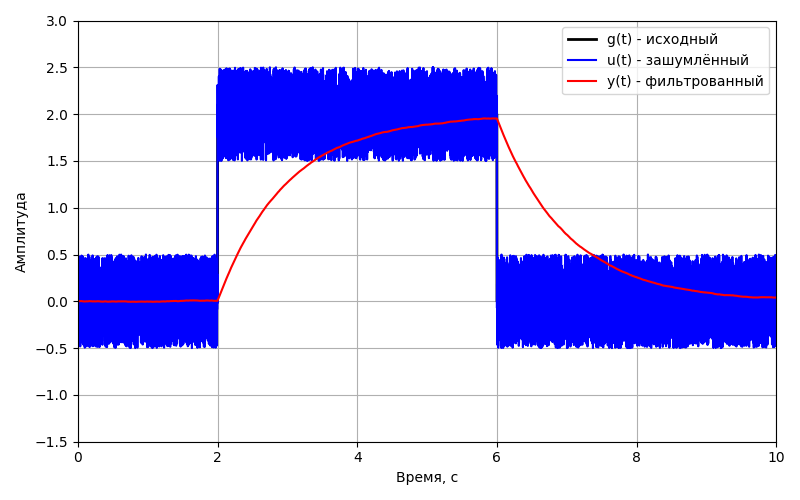
\includegraphics[width=0.8\textwidth]{src/task_1_1/time_2.0_1.0.png}
  \caption{Временные сигналы при \(T=1.0\).}
  \label{fig:time_1.0}
\end{figure}

\begin{figure}[H]
  \centering
  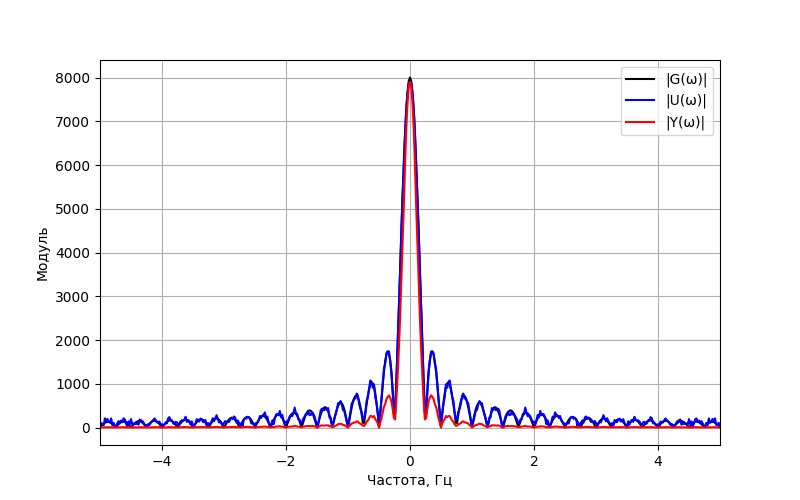
\includegraphics[width=0.8\textwidth]{src/task_1_1/spec_2.0_1.0.png}
  \caption{Спектральные образы сигналов при \(T=1.0\).}
  \label{fig:spec_1.0}
\end{figure}

\begin{figure}[H]
  \centering
  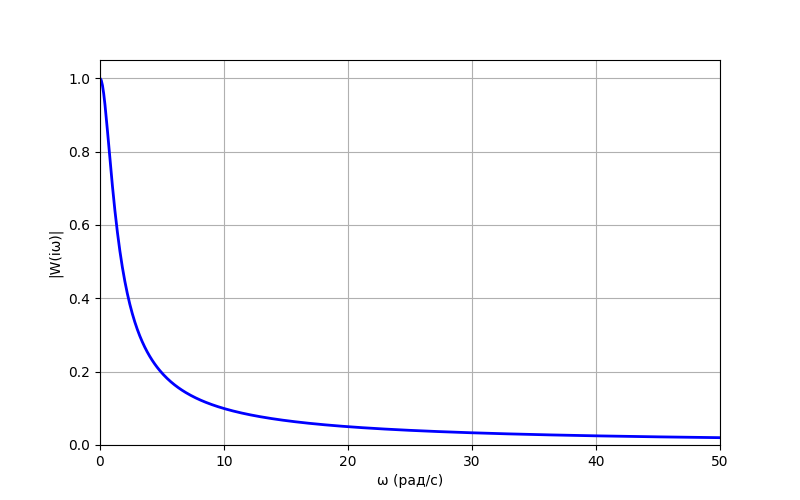
\includegraphics[width=0.8\textwidth]{src/task_1_1/ach_2.0_1.0.png}
  \caption{АЧХ фильтра при \(T=1.0\).}
  \label{fig:ach_1.0}
\end{figure}

\begin{figure}[H]
  \centering
  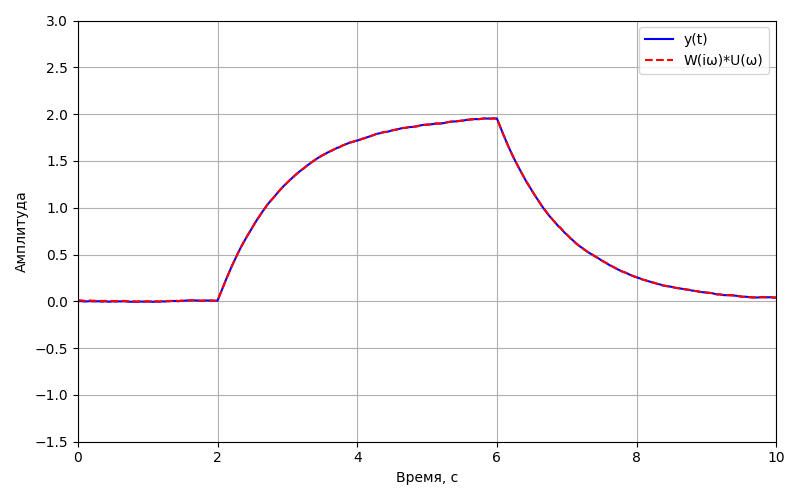
\includegraphics[width=0.8\textwidth]{src/task_1_1/time_comp_2.0_1.0.png}
  \caption{Сравнение временных сигналов для \(T=1.0\).}
  \label{fig:timecomp_1.0}
\end{figure}

\begin{figure}[H]
  \centering
  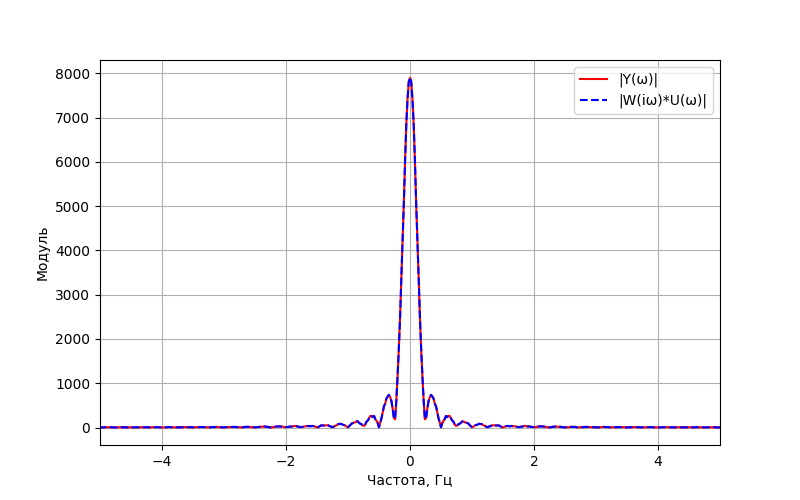
\includegraphics[width=0.8\textwidth]{src/task_1_1/spec_comp_2.0_1.0.png}
  \caption{Сравнение спектральных образов для \(T=1.0\).}
  \label{fig:speccomp_1.0}
\end{figure}

Эксперименты демонстрируют, что при малом значении \(T\) фильтр имеет быстрый отклик, однако шумовые компоненты остаются слабо подавленными. При увеличении \(T\) наблюдается улучшение качества фильтрации за счёт эффективного ослабления высокочастотного шума, что сопровождается некоторой задержкой сигнала.

Но как поведет себя фильтр при увелении амплитуды изначального сигнала? Для этого проведем эксперименты при \(a={4.0, 6.0, 8.0}\) и \(T=0.5\) и посмотрим на рузельтаты.

\begin{figure}[H]
  \centering
  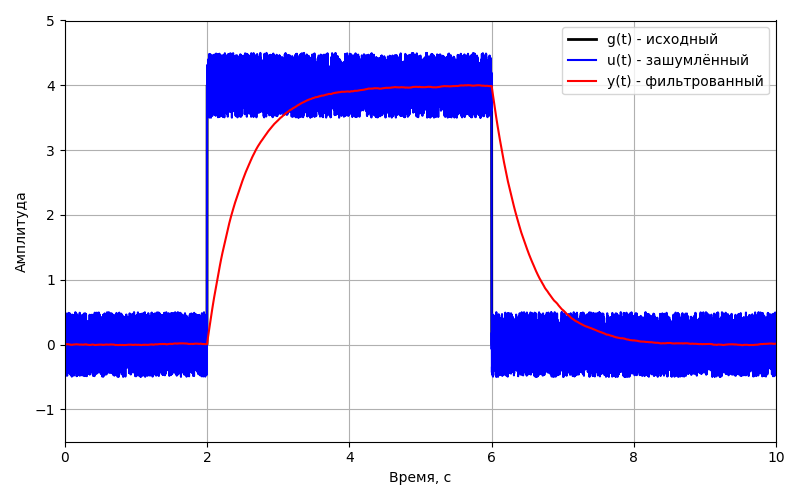
\includegraphics[width=0.8\textwidth]{src/task_1_1/time_4.0_0.5.png}
  \caption{Временные сигналы при \(a=4.0\), \(T=0.5\).}
\end{figure}

\begin{figure}[H]
  \centering
  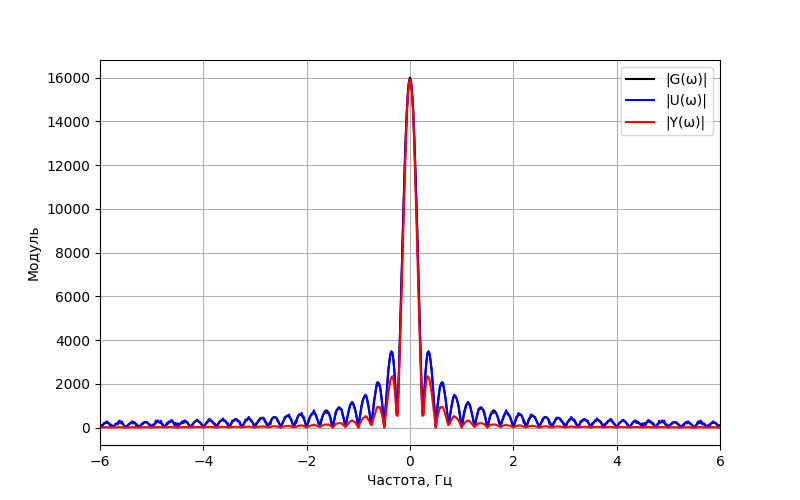
\includegraphics[width=0.8\textwidth]{src/task_1_1/spec_4.0_0.5.png}
  \caption{Спектральный анализ при \(a=4.0\), \(T=0.5\).}
\end{figure}

\begin{figure}[H]
  \centering
  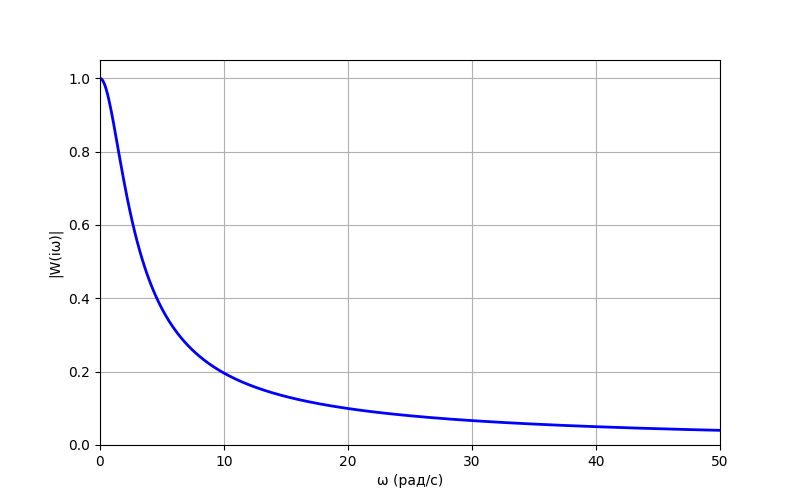
\includegraphics[width=0.8\textwidth]{src/task_1_1/ach_4.0_0.5.png}
  \caption{АЧХ фильтра при \(a=4.0,\ T=0.5\).}
\end{figure}

\begin{figure}[H]
  \centering
  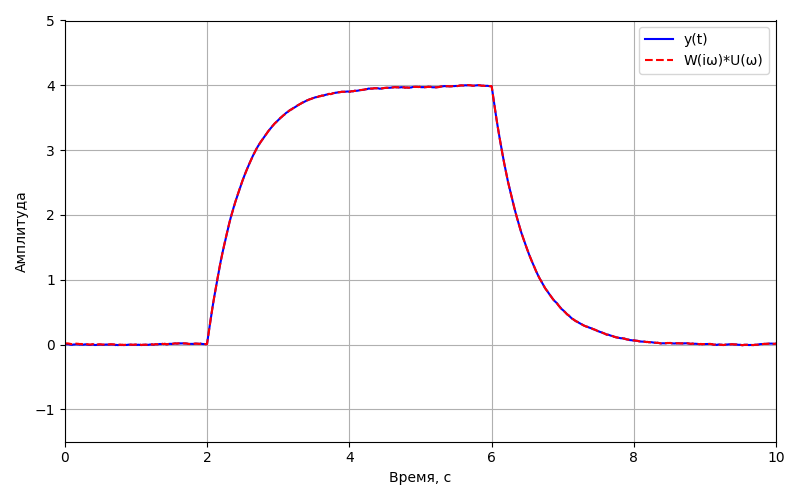
\includegraphics[width=0.8\textwidth]{src/task_1_1/time_comp_4.0_0.5.png}
  \caption{Сравнение временных сигналов при \(a=4.0\), \(T=0.5\).}
\end{figure}

\begin{figure}[H]
  \centering
  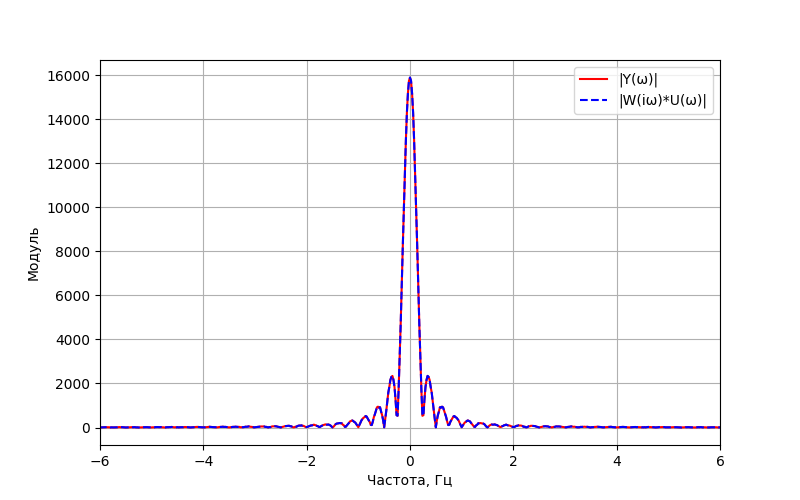
\includegraphics[width=0.8\textwidth]{src/task_1_1/spec_comp_4.0_0.5.png}
  \caption{Сравнение спектральных образов при \(a=4.0\), \(T=0.5\).}
\end{figure}
\noindent Анализ графиков показывает, что при \(T=0.5\) наблюдаются аналогичное поведение, как и для \(a=2.0\). Посмотрим, что будет с фильтром при \(a=6.0\) и \(a=8.0\).

\begin{figure}[H]
  \centering
  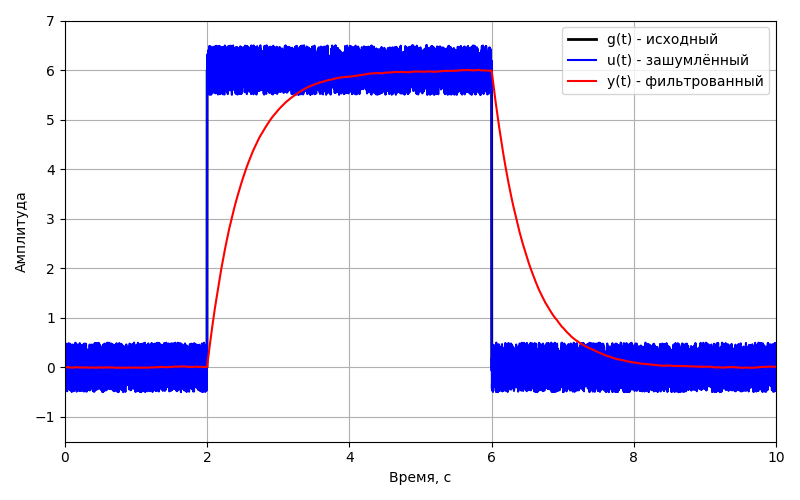
\includegraphics[width=0.8\textwidth]{src/task_1_1/time_6.0_0.5.png}
  \caption{Временные сигналы при $a = 6.0$, $T = 0.5$.}
\end{figure}

\begin{figure}[H]
  \centering
  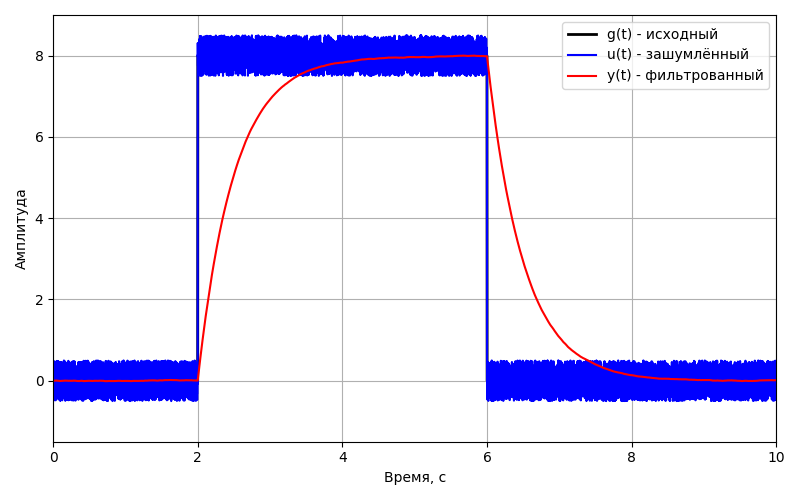
\includegraphics[width=0.8\textwidth]{src/task_1_1/time_8.0_0.5.png}
  \caption{Временные сигналы при \(a=8.0\), \(T=0.5\).}
\end{figure}

\noindent При \(a=6.0\) и \(a=8.0\) наблюдаются увеличения амплитуды исходного сигнала, что приводит к повышению абсолютных значений фильтрованного сигнала. Форма импульса остается схожей с вариантом \(a=4.0\), однако общая динамика сигнала возрастает.

\begin{figure}[H]
  \centering
  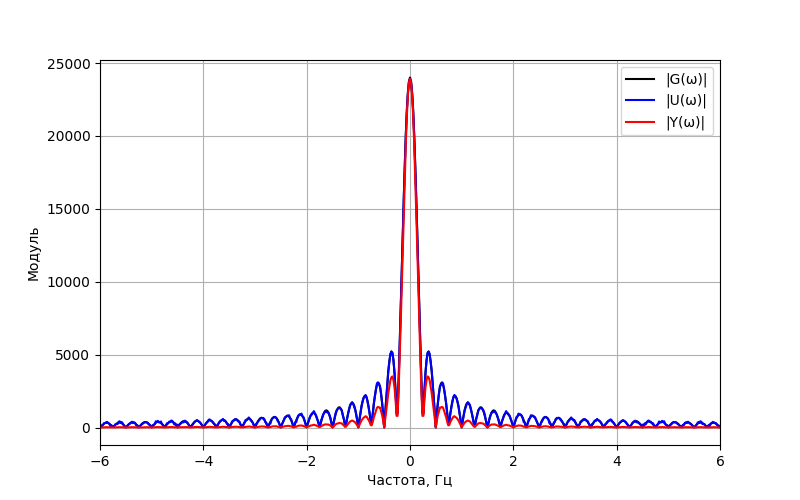
\includegraphics[width=0.8\textwidth]{src/task_1_1/spec_6.0_0.5.png}
  \caption{Спектральный анализ при $a = 6.0$, $T = 0.5$.}
\end{figure}

\begin{figure}[H]
  \centering
  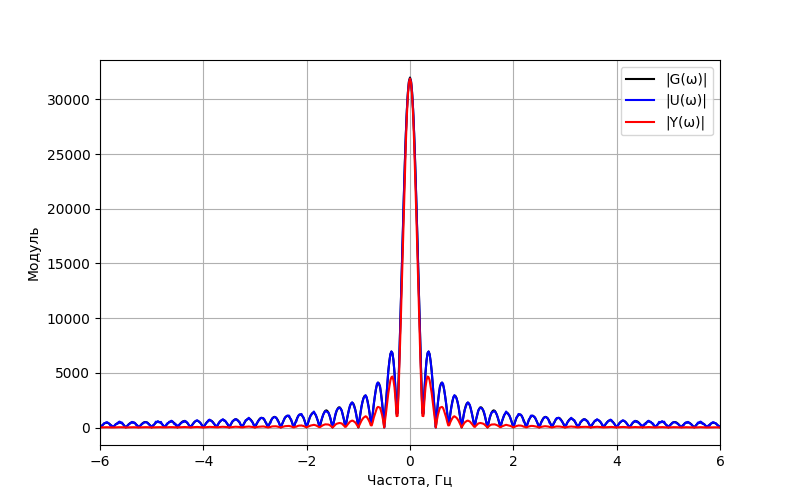
\includegraphics[width=0.8\textwidth]{src/task_1_1/spec_8.0_0.5.png}
  \caption{Спектральный анализ при \(a=8.0\), \(T=0.5\).}
\end{figure}

\begin{figure}[H]
  \centering
  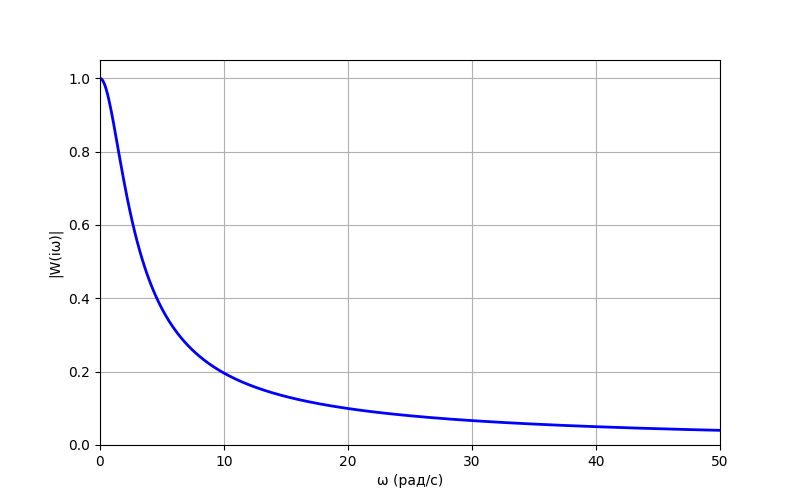
\includegraphics[width=0.8\textwidth]{src/task_1_1/ach_6.0_0.5.png}
  \caption{АЧХ фильтра при $a = 6.0$, $T = 0.5$.}
\end{figure}

\begin{figure}[H]
  \centering
  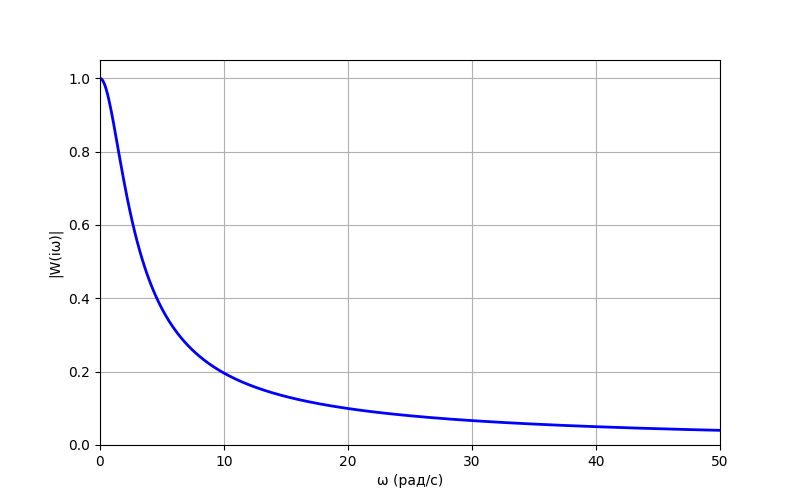
\includegraphics[width=0.8\textwidth]{src/task_1_1/ach_8.0_0.5.png}
  \caption{АЧХ фильтра при $a = 8.0$, $T = 0.5$.}
\end{figure}

\begin{figure}[H]
  \centering
  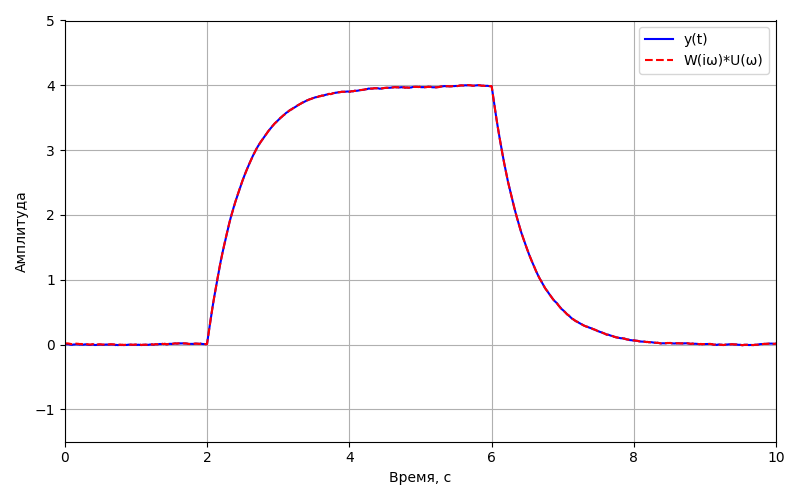
\includegraphics[width=0.8\textwidth]{src/task_1_1/time_comp_4.0_0.5.png}
  \caption{Сравнение временных сигналов при $a = 4.0$, $T = 0.5$.}
\end{figure}

\begin{figure}[H]
  \centering
  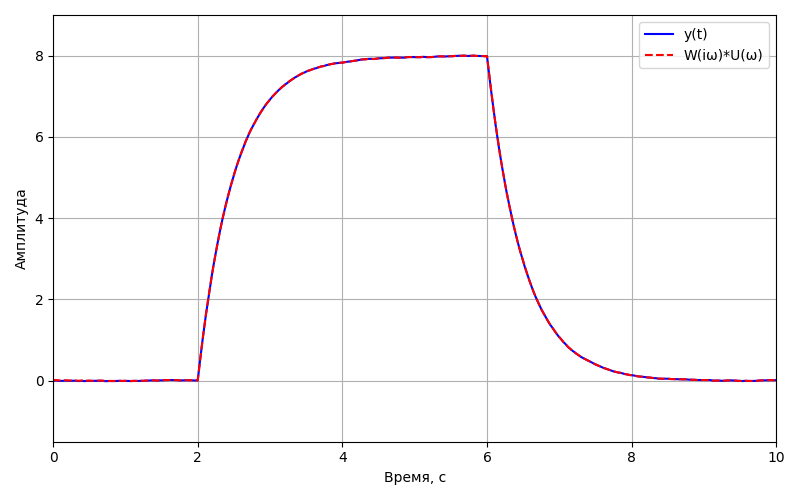
\includegraphics[width=0.8\textwidth]{src/task_1_1/time_comp_8.0_0.5.png}
  \caption{Сравнение временных сигналов при \(a=8.0\), \(T=0.5\).}
\end{figure}

\begin{figure}[H]
  \centering
  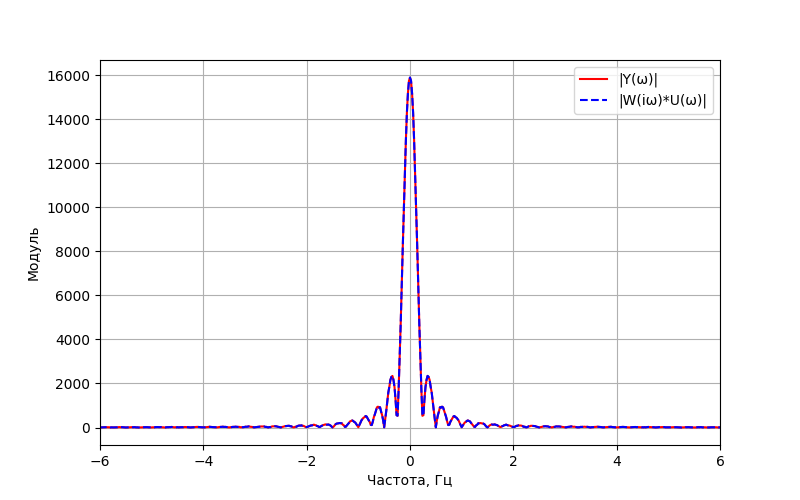
\includegraphics[width=0.8\textwidth]{src/task_1_1/spec_comp_4.0_0.5.png}
  \caption{Сравнение спектральных образов при $a = 4.0$, $T = 0.5$.}
\end{figure}

\begin{figure}[H]
  \centering
  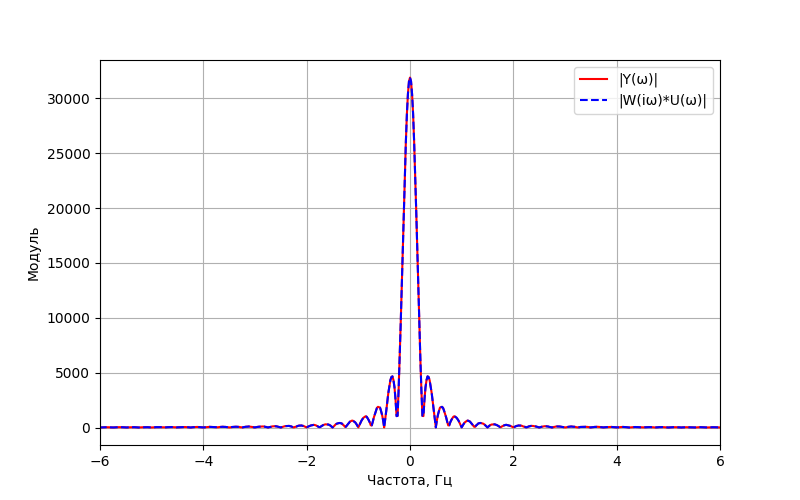
\includegraphics[width=0.8\textwidth]{src/task_1_1/spec_comp_8.0_0.5.png}
  \caption{Сравнение спектральных образов при \(a=8.0\), \(T=0.5\).}
\end{figure}

\noindent На графиках сравнения временных сигналов и спектральных образов видно, что результаты, полученные методом \texttt{lsim} и через обратное Фурье-преобразование, совпадают. Это подтверждает корректность реализации фильтрации как в временной, так и в частотной областях. 

\paragraph{Вывод}
Анализ графиков показывает, что фильтр \(W_1(p)=\frac{1}{Tp+1}\) эффективно уменьшает высокочастотный шум, однако его работа зависит от значения параметра \(T\). При малом \(T=0.1\) фильтр имеет быстрый отклик, но шум остается достаточно выраженными. Увеличение \(T\) до \(0.5\) и \(1.0\) приводит к более эффективному шумоподавлению, однако сопровождается заметной задержкой сигнала. При увеличении амплитуды сигнала до \(a=4.0\) наблюдается, что качество сглаживания остается неизменным. 

Таким образом, оптимальный выбор \(T\) определяется компромиссом между скоростью отклика и степенью подавления шума. На основе экспериментов делаем вывод, что диапазон \(T \approx 0.5\) обеспечивает достаточное сглаживание при приемлемой задержке сигнала.

\addsubsection{Фильтр второго порядка}

В этом пункте мы исследуем применение режекторного полосового фильтра для подавления гармонической составляющей в сигнале. Исходный сигнал, как в 1 пункте, задаётся прямоугольным импульсом на интервале $[t_1,t_2]$. Основная цель --- разработать фильтр вида
\[
W_2(p)=\frac{p^2+a_1p+a_2}{p^2+b_1p+b_2},
\]
удовлетворяющий следующим условиям:
\begin{itemize}
    \item Фильтр должен быть устойчивым (все корни знаменателя имеют отрицательную действительную часть);
    \item Значение фильтра равно 1 при низких и высоких частотах ($W_2(0)=1$, \quad $\lim_{p \to \infty }W_2(p)=1$);
    \item На целевой частоте происходит режекторный эффект, т.е. $W_2(i\omega_0)=0$.
\end{itemize}

Выведем значение параметров, которые будут соотвествовать нашим свойствам.
Так как на низких и высоких частотах фильтр должен иметь значение 1, то при $p=0$ имеем:
\[
W_2(0)=\frac{a_2}{b_2}=1 \quad\Longrightarrow\quad a_2=b_2.
\]
Значит $a_2=b_2$. Теперь подствавим $p=i\omega_0$ в фильтр и приравняем его к нулю, получаем:
\[
(i\omega_0)^2+a_1(i\omega_0)+a_2=-\omega_0^2+i\,a_1\omega_0+a_2=0.
\]
Для обнуления числителя достаточно выбрать:
\[
a_1=0\quad \text{и} \quad a_2=\omega_0^2.
\]
Так как $a_2=b_2$, то и $b_2=\omega_0^2$. Для устойчивости фильтра необходимо, чтобы все корни знаменателя имели отрицательную действительную часть. Это условие выполняется, если $b_1>0$ и $b_2>0$. Таким образом, мы можем записать:
\[
p^2+b_1p+\omega_0^2 = 0,
\]

Таким образом, итоговый набор параметров получается таким:
\[
a_1=0,\quad a_2=\omega_0^2,\quad b_1=b_1 > 0,\quad b_2=\omega_0^2.
\]
Для проверки фильтра зададим следующие значения:
\begin{itemize}
    \item Исходный сигнал: $a=2.0$, активен на интервале $[t_1,t_2]=[2.0,6.0]$.
    \item Амплитуду синусоидальное возмущения зададим как $c=0.5$, частоту --- $d=4$, а $\omega_0=2$.
    \item Зададим $b_1$ как множество значений $b_1=\{1.0, 3.0, 10.0\}$.
\end{itemize}
Построим графики АЧХ фильтра и посмотрим как параметр $b_1$ влияет на работу.

\begin{figure}[H]
  \centering
  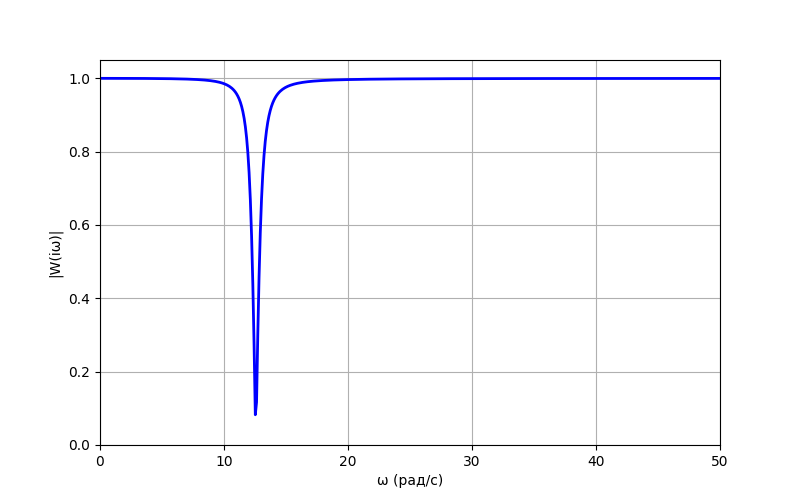
\includegraphics[width=0.8\textwidth]{src/task_1_2/1. ach_157_1_0.5.png}
  \caption{АЧХ фильтра при $a2 = b_2 = 4$, $b_1=1.0$, $c=0.5$, $d=4$.}
\end{figure}
\begin{figure}[H]
  \centering
  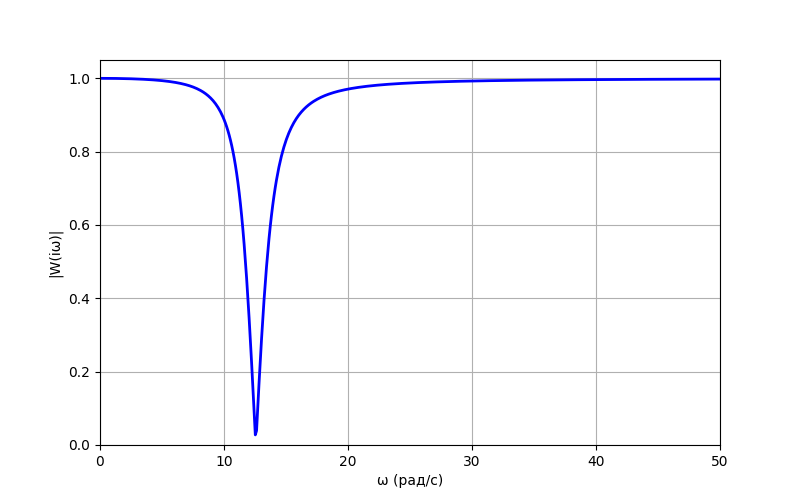
\includegraphics[width=0.8\textwidth]{src/task_1_2/1. ach_157_3_0.5.png}
  \caption{АЧХ фильтра при $a2 = b_2 = 4$, $b_1=3.0$, $c=0.5$, $d=4$.}
\end{figure}
\begin{figure}[H]
  \centering
  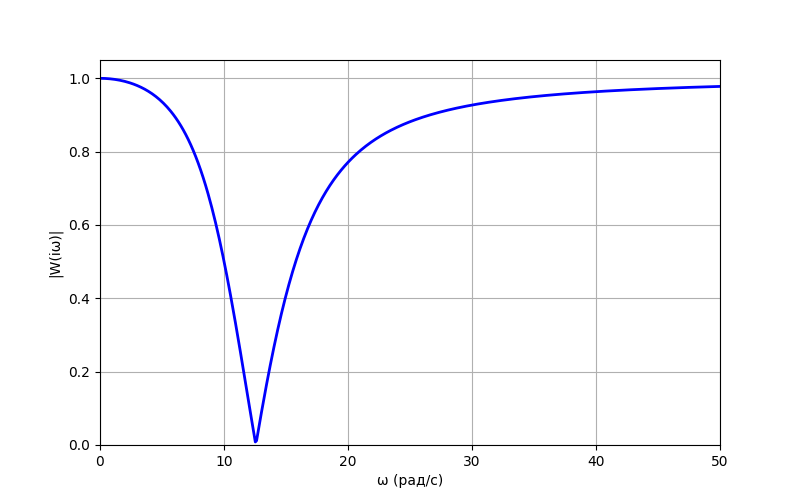
\includegraphics[width=0.8\textwidth]{src/task_1_2/1. ach_157_10_0.5.png}
  \caption{АЧХ фильтра при $a2 = b_2 = 4$, $b_1=10.0$, $c=0.5$, $d=4$.}
\end{figure}
\noindent Глядя на графики АЧХ фильтра можно сделать вывод, что параметр b1 отвечает за ширину полосы пропускания. При увеличении b1 ширина полосы пропускания увеличивается, что приводит к более широкому диапазону частот, которые фильтр пропускает. Это может быть полезно в ситуациях, когда необходимо сохранить больше частотных компонент в выходном сигнале.

Построим графики для временных сигналов, спектров. Также сравним результаты фильтрации, полученные методом \texttt{lsim} и через обратное Фурье-преобразование.
\begin{figure}[H]
  \centering
  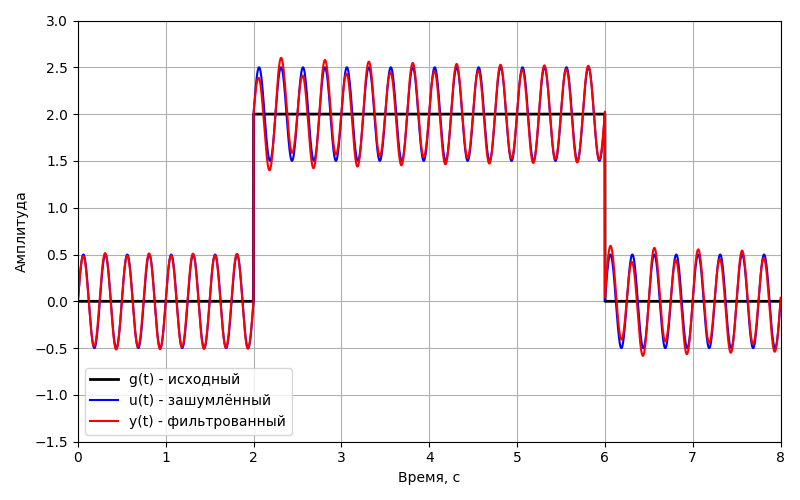
\includegraphics[width=0.8\textwidth]{src/task_1_2/2. time_157_1_0.5.png}
  \caption{Временные сигналы при $a2 = b_2 = 4$, $b_1=1.0$, $c=0.5$, $d=4$.}
\end{figure}

\begin{figure}[H]
  \centering
  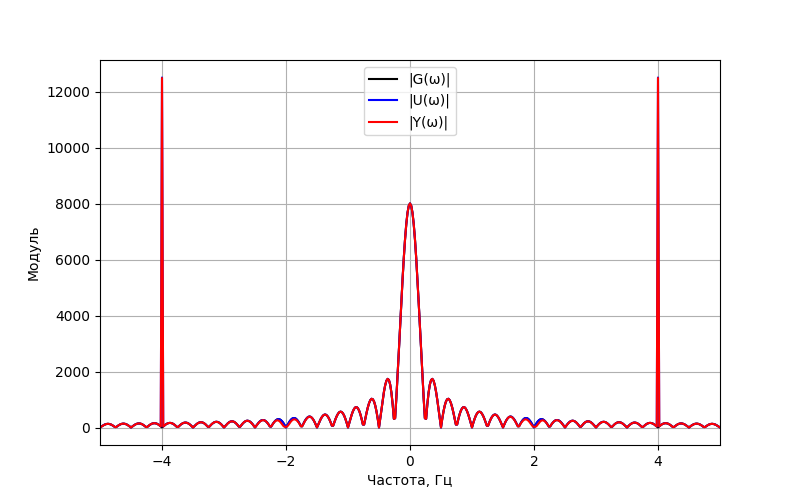
\includegraphics[width=0.8\textwidth]{src/task_1_2/2. spec_157_1_0.5.png}
  \caption{Спектральный анализ при $a2 = b_2 = 4$, $b_1=1.0$, $c=0.5$, $d=4$.}
\end{figure}

\begin{figure}[H]
  \centering
  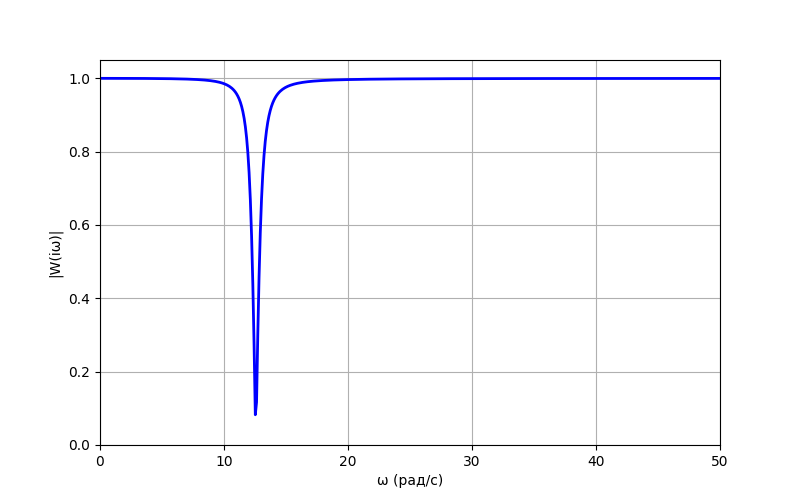
\includegraphics[width=0.8\textwidth]{src/task_1_2/1. ach_157_1_0.5.png}
  \caption{АЧХ фильтра при $a2 = b_2 = 4$, $b_1=1.0$, $c=0.5$, $d=4$.}
\end{figure}

\begin{figure}[H]
  \centering
  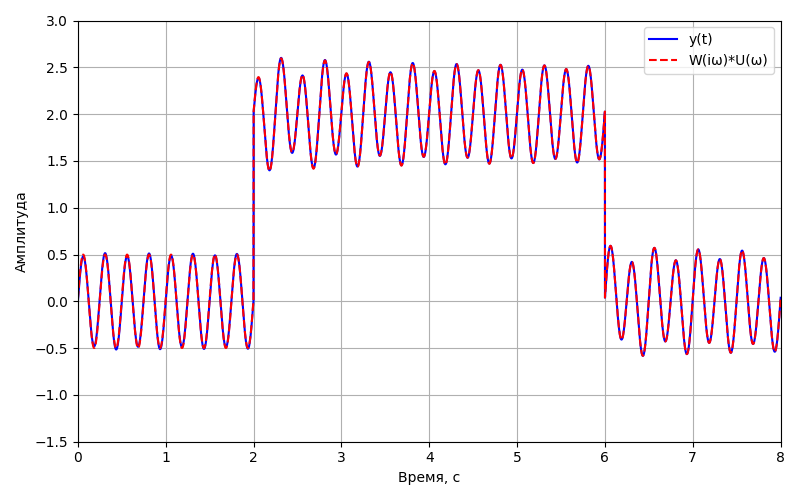
\includegraphics[width=0.8\textwidth]{src/task_1_2/2. time_comp_157_1_0.5.png}
  \caption{Сравнение временных сигналов при $a2 = b_2 = 4$, $b_1=1.0$, $c=0.5$, $d=4$.}
\end{figure}

\begin{figure}[H]
  \centering
  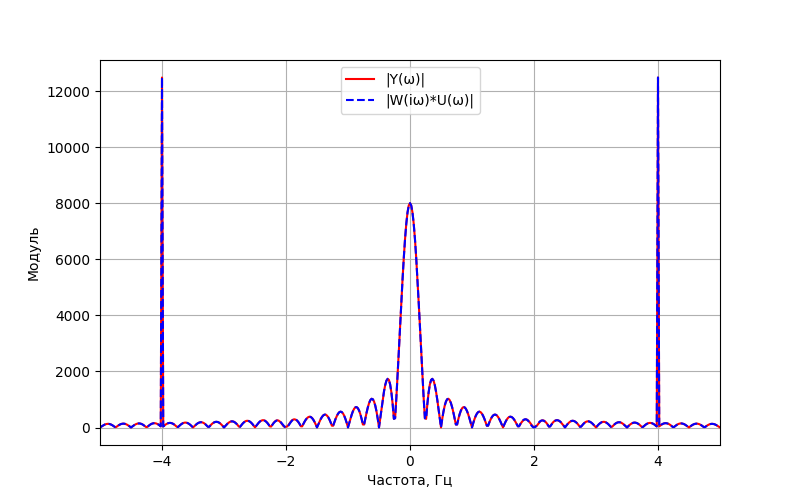
\includegraphics[width=0.8\textwidth]{src/task_1_2/2. spec_comp_157_1_0.5.png}
  \caption{Сравнение спектральных образов при $a2 = b_2 = 4$, $b_1=1.0$, $c=0.5$, $d=4$.}
\end{figure}
\noindent Сравнительный спектральный и временной анализ подтверждают корректность работы фильтра. Но видно, что фильтр не смог погасить синусоидальное возмущение.

Теперь попробуем увеличить ширину работы фильтра посмотрим на графики при $b_1 = 3.0$.  

\begin{figure}[H]
  \centering
  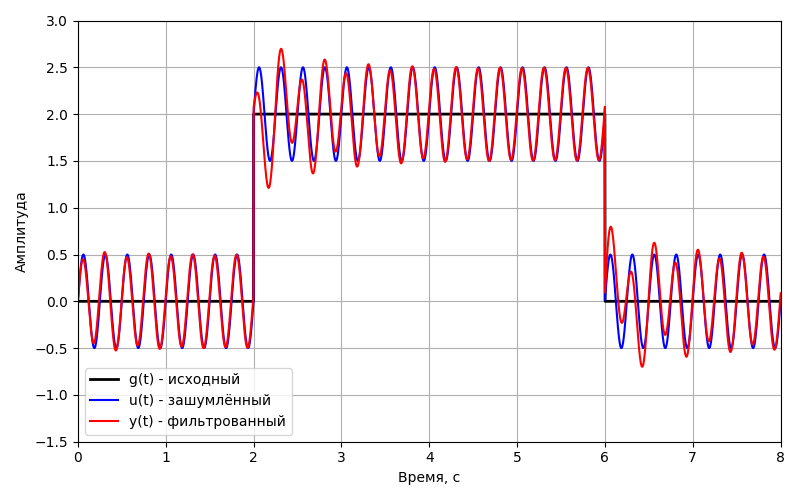
\includegraphics[width=0.8\textwidth]{src/task_1_2/1. time_157_3_0.5.png}
  \caption{Временные сигналы при $a2 = b_2 = 4$, $b_1=3.0$, $c=0.5$, $d=4$.}
\end{figure}
\begin{figure}[H]
  \centering
  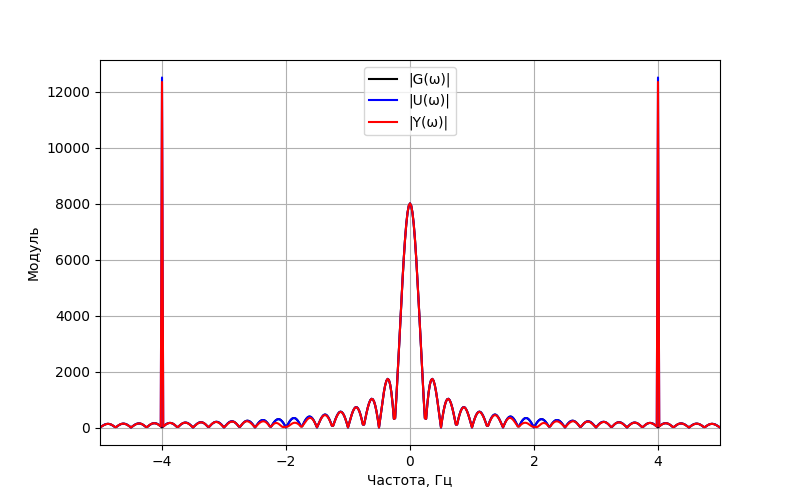
\includegraphics[width=0.8\textwidth]{src/task_1_2/1. spec_157_3_0.5.png}
  \caption{Спектральный анализ ппри $a2 = b_2 = 4$, $b_1=3.0$, $c=0.5$, $d=4$.}
\end{figure}
\begin{figure}[H]
  \centering
  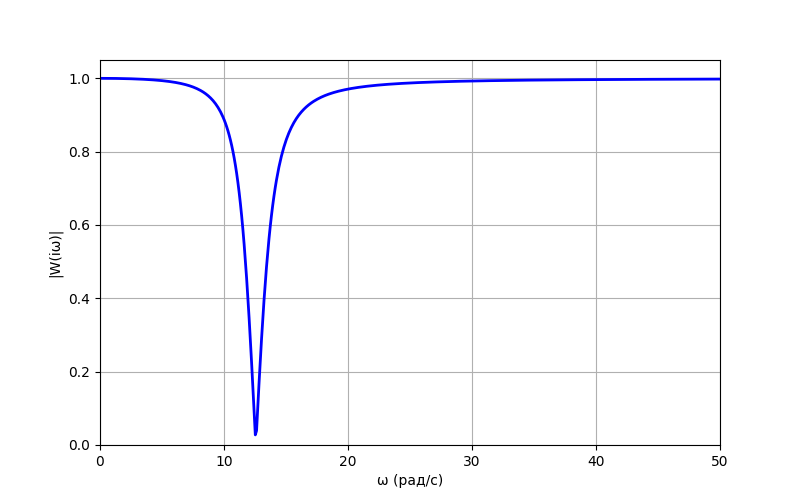
\includegraphics[width=0.8\textwidth]{src/task_1_2/1. ach_157_3_0.5.png}
  \caption{АЧХ фильтра при $a2 = b_2 = 4$, $b_1=3.0$, $c=0.5$, $d=4$.}
\end{figure}
\begin{figure}[H]
  \centering
  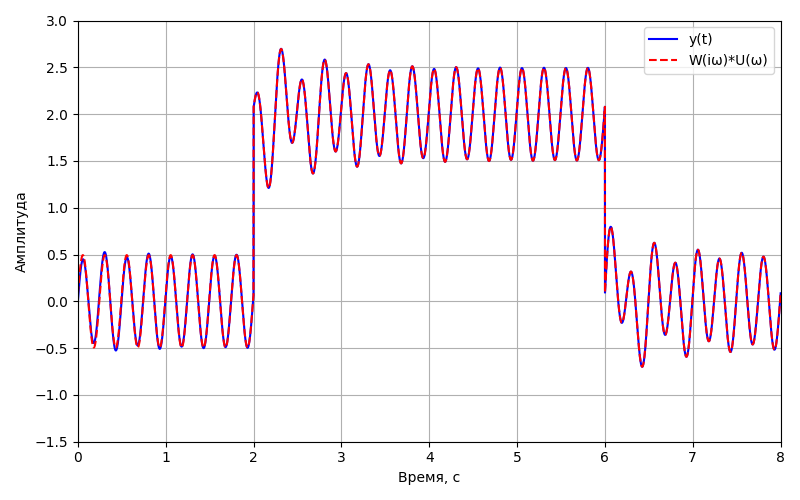
\includegraphics[width=0.8\textwidth]{src/task_1_2/1. time_comp_157_3_0.5.png}
  \caption{Сравнение временных сигналов при $a2 = b_2 = 4$, $b_1=3.0$, $c=0.5$, $d=4$.}
\end{figure}

Уже лучше, но фильтр не справляется с синусоидальным возмущением. Если посмотреть на графики спектров, то можно заметить, что присутсвует большой скачок в области 4 Гц. Попробуем оставить параметр $b_1 = 3.0$ и изменить частоту синусоидального возмущения, например, на $d = 1$. Посмотрим на графики:

\begin{figure}[H]
  \centering
  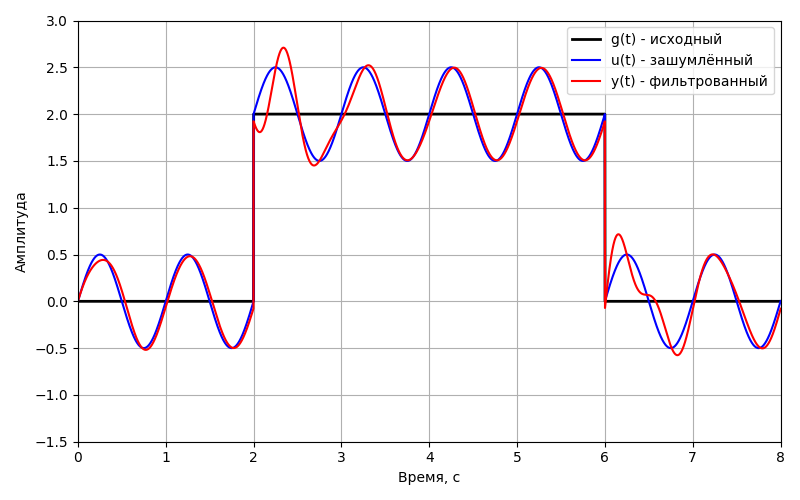
\includegraphics[width=0.8\textwidth]{src/task_1_2/4. time_157_3_0.5.png}
  \caption{Временные сигналы при $a2 = b_2 = 4$, $b_1=3.0$, $c=0.5$, $d=1$.}
\end{figure}
\begin{figure}[H]
  \centering
  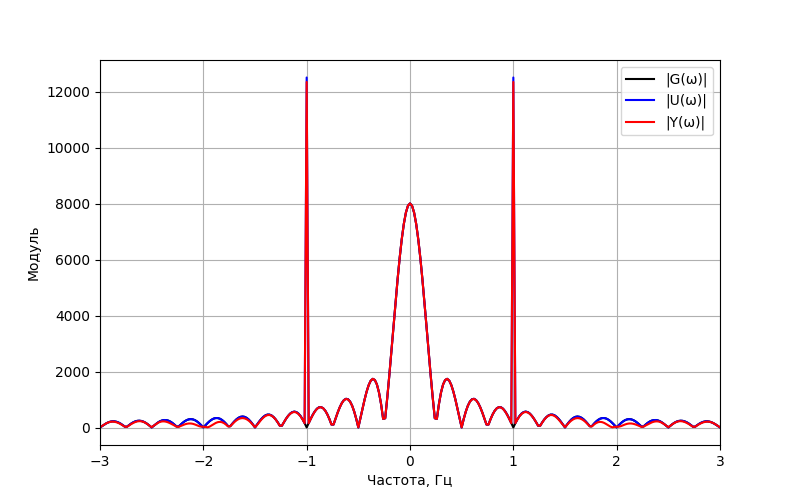
\includegraphics[width=0.8\textwidth]{src/task_1_2/4. spec_157_3_0.5.png}
  \caption{Спектральный анализ ппри $a2 = b_2 = 4$, $b_1=3.0$, $c=0.5$, $d=1$.}
\end{figure}
\begin{figure}[H]
  \centering
  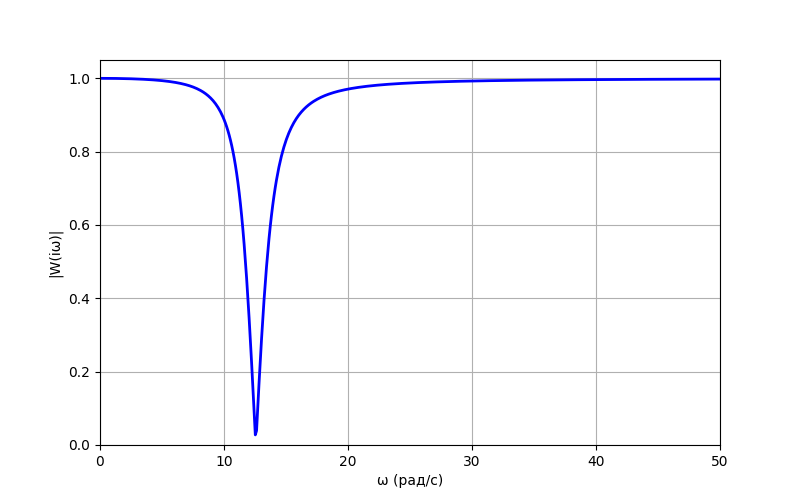
\includegraphics[width=0.8\textwidth]{src/task_1_2/4. ach_157_3_0.5.png}
  \caption{АЧХ фильтра при $a2 = b_2 = 4$, $b_1=3.0$, $c=0.5$, $d=1$.}
\end{figure}
\begin{figure}[H]
  \centering
  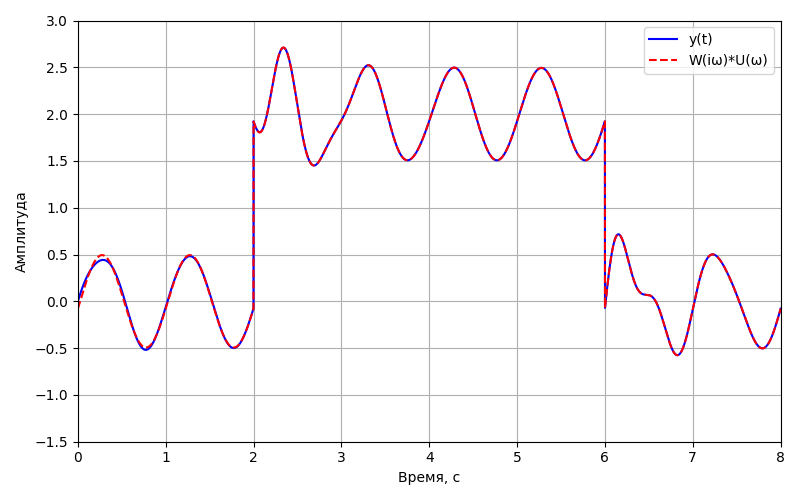
\includegraphics[width=0.8\textwidth]{src/task_1_2/4. time_comp_157_3_0.5.png}
  \caption{Сравнение временных сигналов при $a2 = b_2 = 4$, $b_1=3.0$, $c=0.5$, $d=1$.}
\end{figure}

Как мы видим основной шум переместился в область 1 Гц, а синусоидальное возмущение стало менее заметным. Теперь попробуем увеличить частоту синусоидального возмущения до 2 Гц и посмотрим на графики:

\begin{figure}[H]
  \centering
  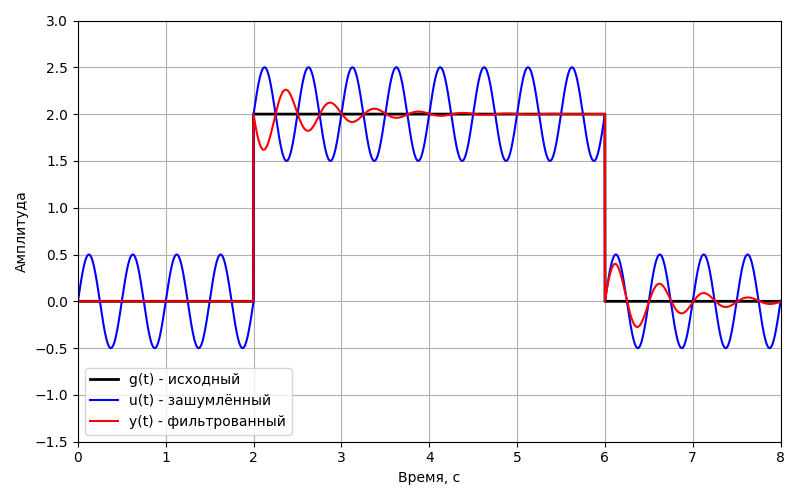
\includegraphics[width=0.8\textwidth]{src/task_1_2/5. time_157_3_0.5.png}
  \caption{Временные сигналы при $a2 = b_2 = 4$, $b_1=3.0$, $c=0.5$, $d=2$.}
\end{figure}
\begin{figure}[H]
  \centering
  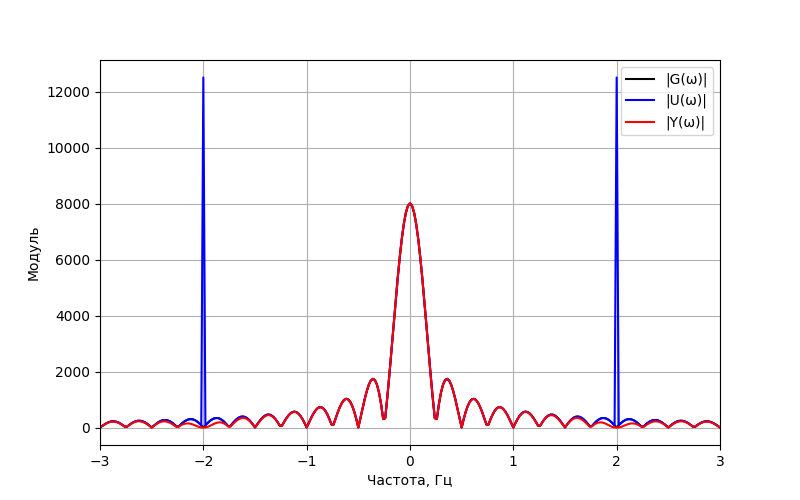
\includegraphics[width=0.8\textwidth]{src/task_1_2/5. spec_157_3_0.5.png}
  \caption{Спектральный анализ ппри $a2 = b_2 = 4$, $b_1=3.0$, $c=0.5$, $d=2$.}
\end{figure}
\begin{figure}[H]
  \centering
  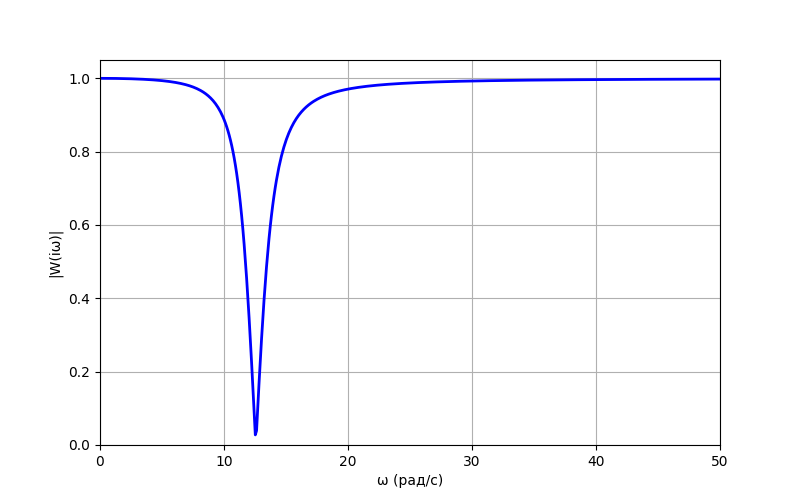
\includegraphics[width=0.8\textwidth]{src/task_1_2/5. ach_157_3_0.5.png}
  \caption{АЧХ фильтра при $a2 = b_2 = 4$, $b_1=3.0$, $c=0.5$, $d=2$.}
\end{figure}
\begin{figure}[H]
  \centering
  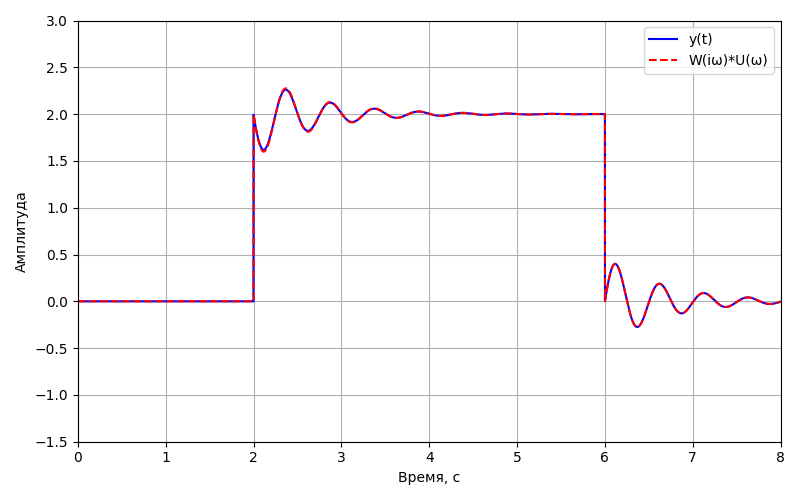
\includegraphics[width=0.8\textwidth]{src/task_1_2/5. time_comp_157_3_0.5.png}
  \caption{Сравнение временных сигналов при $a2 = b_2 = 4$, $b_1=3.0$, $c=0.5$, $d=2$.}
\end{figure}

\noindent На графиках мы видим, что фильтр подавил практически весь шум. Это произошло в момент, когда $d=\omega_0$. Стоит отметь, что результаты, полученные методом lsim, и сигналы, рассчитанные через обратное преобразование произведения, полностью совпадают, что подтверждает корректность реализации фильтра.

Теперь попробуем увеличить амплитуду колебаний $c=1.0$, остальные параметры оставим неизменными. Посмотрим как отработает фильтр.

\begin{figure}[H]
  \centering
  \includegraphics[width=0.8\textwidth]{src/task_1_2/6. time_157_3_1.0.png}
  \caption{Временные сигналы при $a2 = b_2 = 4$, $b_1=3.0$, $c=1.0$, $d=2$.}
\end{figure}
\begin{figure}[H]
  \centering
  \includegraphics[width=0.8\textwidth]{src/task_1_2/6. spec_157_3_1.0.png}
  \caption{Спектральный анализ ппри $a2 = b_2 = 4$, $b_1=3.0$, $c=1.0$, $d=2$.}
\end{figure}
\begin{figure}[H]
  \centering
  \includegraphics[width=0.8\textwidth]{src/task_1_2/6. ach_157_3_1.0.png}
  \caption{АЧХ фильтра при $a2 = b_2 = 4$, $b_1=3.0$, $c=1.0$, $d=2$.}
\end{figure}
\begin{figure}[H]
  \centering
  \includegraphics[width=0.8\textwidth]{src/task_1_2/6. time_comp_157_3_1.0.png}
  \caption{Сравнение временных сигналов при $a2 = b_2 = 4$, $b_1=3.0$, $c=1.0$, $d=2$.}
\end{figure}
\noindent При увеличении амплитуды возмущения синусоидальные колебания во временных сигналах становятся более заметными. Однако, несмотря на это, фильтр по-прежнему успешно справляется с задачей удаления высокочастотного шума. Временные сигналы показывают, что синусоидальная составляющая становится более выраженной, но фильтр продолжает эффективно подавлять её.

\paragraph{Вывод} Анализ полученных графиков позволяет сделать следующие выводы:
\begin{itemize}
    \item Базовый набор параметров ($a1=0.0$, $a2 = b_2 = 4$, $b1 = 3.0$) обеспечивает эффективное подавление нежелательной гармонической составляющей при целевой частоте 2 Гц, что подтверждается глубоким и узким провалом в спектральном анализе и корректной АЧХ.
    \item При увеличении амплитуды возмущения ($c=1.0$) наблюдаются более выраженные колебания во временных сигналах, но это не влияет на эффективность фильтра.
    \item Варирование значения параметра $b_1$ существенно влияет на ширину режекторной полосы: при низком значении $b_1$ подавляется узкий диапазон частот, а при высоком значении провал становится очень широким, что может привести к фазовым искажениям. Оптимальное значение, полученное экспериментально, оказалось около $b_1=3.0$.
\end{itemize}

Таким образом, режекторный фильтр с передаточной функцией $W_2(p)$ при оптимально подобранных параметрах, способен эффективно подавлять нежелательные гармоники, сохраняя при этом форму полезного сигнала. 

\addsection{Задание 2. Сглаживание биржевых данных}
В данном задании требуется представить метод сглаживания биржевых котировок, где степень сглаживания зависит от рассматриваемого временного периода. Сглаживание осуществляется с помощью линейного фильтра первого порядка, реализованного в Python, что позволяет смягчить кратковременный разброс цен и представить данные в более наглядном виде для анализа. В работе использованы данные по котировкам акций СберБанка в период с 01.01.2021 по 31.03.2025.

\begin{figure}[H]
  \centering
  \includegraphics[width=0.9\textwidth]{src/orig_price.png}
  \caption{Исходные биржевые котировки.}
\end{figure}
\noindent На данном графике представлена динамика биржевых котировок до применения сглаживающего фильтра. Наблюдаются значительные кратковременные колебания, что затрудняет выявление долгосрочных трендов.

Для сглаживания использовался фильтр первого порядка. Фильтрация проводилась для различных значений \(T\) (соответствующих 1 дню, 7 дням, 30 дням, 90 дням и 365 дням), что позволило оценить, как меняется сглаживание биржевых котировок при изменении временного интервала.

Ниже приведены графики исходных и сглажённых данных.

\begin{figure}[H]
  \centering
  \includegraphics[width=0.9\textwidth]{src/smooth_price_1.png}
  \caption{Сглаживание котировок при \(T=1\) дн.}
\end{figure}
\noindent При сглаживании за один день наблюдается небольшое сглаживание кратковременных колебаний, однако высокочастотные шумовые составляющие остаются заметными. Это говорит о том, что временной интервал сглаживания недостаточен для выделения долгосрочного тренда.

\begin{figure}[H]
  \centering
  \includegraphics[width=0.9\textwidth]{src/smooth_price_7.png}
  \caption{Сглаживание котировок при \(T=7\) дн.}
\end{figure}
\noindent При сглаживании за 7 дней наблюдается более выраженное сглаживание, что позволяет выделить краткосрочный тренд.

\begin{figure}[H]
  \centering
  \includegraphics[width=0.9\textwidth]{src/smooth_price_30.png}
  \caption{Сглаживание котировок при \(T=30\) дн.}
\end{figure}
\noindent Сглаживание за 30 дней позволяет значительно убрать кратковременные колебания, демонстрируя общую тенденцию изменения цен. Этот вариант сглаживания особенно полезен для выявления месячных трендов и общего направления рынка.

\begin{figure}[H]
  \centering
  \includegraphics[width=0.9\textwidth]{src/smooth_price_90.png}
  \caption{Сглаживание котировок при \(T=90\) дн.}
\end{figure}
\noindent При сглаживании за 90 дней наблюдается ещё более выраженное сглаживание, которое позволяет увидеть долгосрочные тенденции. Высокочастотные колебания практически исчезают, а общий тренд становится хорошо заметен.

\begin{figure}[H]
  \centering
  \includegraphics[width=0.9\textwidth]{src/smooth_price_365.png}
  \caption{Сглаживание котировок при \(T=365\) дн.}
\end{figure}
\noindent Сглаживание за 365 дней даёт наиболее сглажённую кривую, которая отражает глобальные долгосрочные тренды. При таком уровне сглаживания почти все краткосрочные колебания устраняются, однако может быть потеряна детализация динамики на промежуточных интервалах.

\paragraph{Вывод}
Таким образом, представленный метод сглаживания биржевых котировок демонстрирует, как изменение параметра \(T\) влияет на степень сглаживания, позволяя адаптировать подход под конкретные аналитические задачи.

\addsection{Заключение}

В ходе выполнения лабораторной работы были изучены методы линейной фильтрации, направленные на подавление нежелательных компонентов сигнала. Экспериментальный анализ показал, что правильный выбор параметров позволяет добиться существенного снижения шума и сохранения формы исходного сигнала. \\[0.5em]
Во второй части работы реализовано сглаживание биржевых котировок, где применение линейного фильтра позволяет устранить кратковременные выбросы и выделить долгосрочные тренды. Анализ графиков для различных значений параметра сглаживания продемонстрировал, что чем больше значение T, тем сильнее сглаживается сигнал, однако при слишком высоких значениях теряется детализация краткосрочной динамики. \\[0.5em]
В целом, проведённая работа продемонстрировала эффективность линейных фильтров для обработки сигналов и подтверждает важность тонкой настройки параметров фильтрации.
\end{document}